\documentclass{article}
\author{Bruno Berastain}
\usepackage{amsmath, amssymb, amsthm, tikz}

\begin{document}
\title{Using K-Nearest Neighbors and Linear Regression to Predict Housing Prices}
\maketitle

\section{The Problem}
You're planning to move and it's time to sell your house. You want to set the highest price that will sell quickly. Price it too high, it will take a long time to sell. Price it too low, and you'll get less than the house is worth. How can you find the perfect price?

\section{Compare To Similar Houses}
% sub-section header: K-Nearest Neighbors
What if you looked at recently sold houses similar to yours? That would give you an idea of the price to list your house. Say you had information about 10 recently sold houses, including the prices at which they sold. You could find the house most similar to yours, and assume that your house would sell at the same price. How do you decide which house is most similar to yours? You could take a feature of the houses, like number of rooms, and organize them all on a number line from least to most rooms. Then you could put your house on the number line, and choose the same selling price as the house closest to yours.\\

% how do I make this a dotplot?

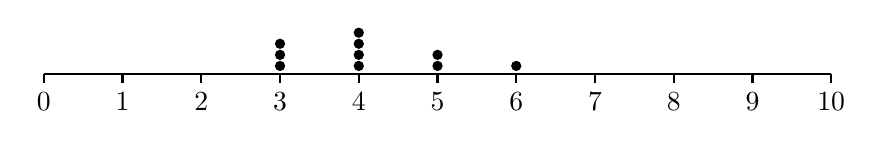
\begin{tikzpicture}[thick]
  \draw(0,0)--(10,0);
  \foreach \x in {0,1,...,10}
    \draw(\x,0pt)--(\x,-3pt) node[below] {\x};
  \foreach \x in {3,4,5,6}
  	\draw [fill] (\x,3pt) circle [radius=0.05];
  \foreach \x in {3,4,5}
  	\draw [fill] (\x,7pt) circle [radius=0.05];
  \foreach \x in {3,4}
  	\draw [fill] (\x,11pt) circle [radius=0.05];
  \draw [fill] (4,15pt) circle [radius=0.05];
\end{tikzpicture}

\\If your house has 4 rooms, you could pick the selling price of one of the other houses with 4 rooms. A better method would be to take the average selling price of all the houses with 4 rooms.\\

Obviously this isn't the N, let's say we also know the number of bedrooms in all 10 houses. 

% We could imagine a graph with the square footage on one axis, and the number of bedrooms on the other. Once again, we can plot all 100 houses. Once again, you can pick the closest one, and assume that your house is worth the same amount. This time, the distance between your house and every other house on the graph follows the equation

% square root of (x1 - x2)^2 + (y1-y2)^2




% should we regularize the 

% The set of 100 houses with known selling price that we used to determine our price is called the training set.
% The price, the variable we are trying to predict, is the target variable.
% All the aspects of the house 



\end{document}